\documentclass[12pt]{article}
\usepackage{amsmath}
\usepackage{mathtools}
\usepackage{amsfonts}
\usepackage{lastpage}
\usepackage{tikz}
\usepackage{pdfpages}
\usepackage{gauss}
\usepackage{fancyvrb}
\usepackage{fancyhdr}
\usepackage{graphicx}
\pagestyle{fancy}
\fancyfoot[C]{\footnotesize Page \thepage\ of 15}
\DeclareGraphicsExtensions{.pdf,.png,.jpg}
\title{Database and Web Programming}
\author{Nikolaj Dybdahl Rathcke}
\chead{Nikolaj Dybdahl Rathcke - rfq695}

\begin{document}

\section*{Modeling}
\subsection*{1.1}
\subsection*{a}
Analyze the database and make changes necessary to bring the data into Boyce/Codd Normal Form (thus also into First, Second and Third Normal Form). Draw an E/R model showing the normalized database model, using the kind of model used in the book with entities as rectangles, attributes as ovals and relationship as diamonds connecting entities. The model must visualize the primary keys. Explain what you changed and why.\\
\\
Nothing is changed, but here is an E/R model of the database:
\\
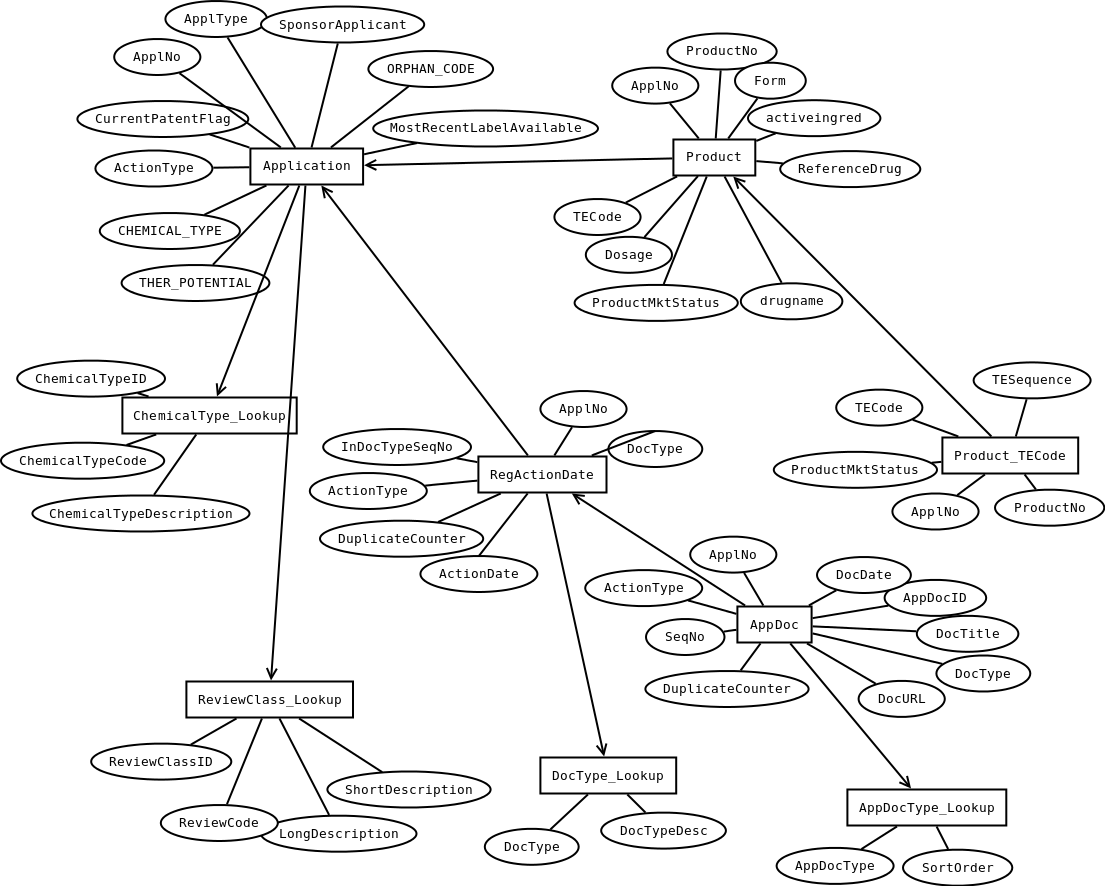
\includegraphics[scale=0.3]{Diagram.png}

\subsection*{b}
Transform your E/R model into a relational schema. We want to keep information about primary keys in the schema. Foreign keys must be described explicit, like this:\\
$$mytable(id, name, department)$$
$$FK: department \rightarrow dept(id)$$
\\
The relational schema looks like this:\\
\\
Application(\underline{ApplNo}, ApplType, SponsorApplicant, MostRecentLabelAvailable, CurrentPatentFlag, ActionType, CHEMICAL\_TYPE, THER\_POTENTIAL, ORPHAN\_CODE)\\
\\
Product(\underline{ApplNo}, \underline{ProductNo}, Form, 	Dosage, \underline{ProductMktStatus}, TECode, ReferenceDrug, drugname, activeingred)\\ 
FK: ApplNo $\rightarrow$ Application(ApplNo)\\ 
\\
Product\_TECode(\underline{ApplNo}, \underline{ProductNo}, TECode, \underline{TESequence}, \underline{ProductMktStatus})\\
FK: ApplNo $\rightarrow$ Product(ApplNo)\\
FK: ProductNo $\rightarrow$ Product(ProductNo)\\
FK: ProductMktStatus $\rightarrow$ Product(ProductMktStatus)\\
\\
ChemicalType\_Lookup(\underline{ChemicalTypeID}, ChemicalTypeCode, ChemicalTypeDescription)\\
\\
RegActionDate(\underline{ApplNo}, ActionType, \underline{InDocTypeSeqNo}, \underline{DuplicateCounter}, ActionDate, DocType)\\
FK: ApplNo $\rightarrow$ Application(ApplNo)\\
\\
AppDoc(\underline{AppDocID}, ApplNo, SeqNo, DocType, DocTitle, DocURL, DocDate, ActionType, DuplicateCounter)\\
\\
ReviewClass\_Lookup(\underline{ReviewClassID}, ReviewCode, LongDescription, ShortDescription)\\
\\
DocType\_Lookup(\underline{DocType}, DocTypeDesc)\\
\\
AppDocType\_Lookup(\underline{AppDocType}, SortOrder)

\subsection*{c}
Make a SQL script (a file) with the SQL statements that can create a database from the relational schema in (b. The SQL script should, beside the table definitions, also define primary and foreign keys and not null constraints.\\
\\
Not assessed.

\section*{Functional dependencies and normalization}
\subsection*{2.1}
Given a relation R(A,B,C,D,E,F). For each set of dependencies (a), (b), (c) find candidate key(s) and normalize to BCNF
$$a)\: A\rightarrow DE, B\rightarrow F, AB\rightarrow C$$
We see that A and B are never mentioned in the right side of the dependencies, therefore they have to be a part of the candidate key as minimum.\\
We also see that we can get following superkey:\\
ABCF (A $\rightarrow$ DE)\\
By trimming down, we can get:\\
ABC (B $\rightarrow$ F)\\
And finally:\\
AB (AB $\rightarrow$ C)\\
Which means AB is the candidate key for the relation R.\\
\\
Now we want to normalize it to BCNF.\\
\\
Since $A\rightarrow DE$ is a violation to BCNF in R since it doesn't contain the candidate key we found, we find the closures of A in R which is,
$$R1=\{A,D,E\}$$
Since there are no occurences of D or E on the left side, we find S1:
$$S1=(\{A,D,E\},\:\{A \rightarrow DE\})$$
Which satisfies BCNF.\\
Then R2 is $R-R1+{A}$:
$$R2=\{A,B,C,F\}$$
$$S2=(\{A,B,C,F\},\:\{B\rightarrow F, AB\rightarrow C\})$$
From S2 we observe that $B\rightarrow F$ is a violation of BCNF. We follow the algorithm and get:
$$R3=\{B,F\}$$
We project the FD's from S2 on R3 and R4:
$$S3=(\{B,F\},\:\{B\rightarrow F\})$$
Which satisfies BCNF.\\
And the remaining:
$$R4=\{A,B,C\}$$
$$S4=(\{A,B,C\},\:\{AB\rightarrow C\})$$
Which satisfies BCNF.
$$S1=(\{A,D,E\},\:\{A \rightarrow DE\})$$
$$S3=(\{B,F\},\:\{B\rightarrow F\})$$
$$S4=(\{A,B,C\},\:\{AB\rightarrow C\})$$
The relation is normalized in these schemas.

$$b)\: AB\rightarrow C, BD\rightarrow EF$$
Again, we see that A, B and D are never mentioned on the right side, so they have to be included in the candidate key as a minimum.\\
We can get following superkey:\\
ABDEF (AB $\rightarrow$ C)\\
Which can be trimmed down to:\\
ABD (BD $\rightarrow$ EF)\\
Therefore ABD is the candidate key, since it can't be trimmed further down.\\
\\
Now we want to normalize it to BCNF.\\
\\
We see that $AB\rightarrow C$ is a violation of BCNF. So we find the closures of AB in R:
$$R1=\{A,B,C\}$$
Since there no occurences of C on the left side in the other FD's, we can determine S1:\\
$$S1=(\{A,B,C\},\:\{AB\rightarrow C\})$$
Which satisfies BCNF.\\
Then R2 is $R-R1+{A,B}$:
$$R2=\{A,B,D,E,F\}$$
$$S2=(\{A,B,D,E,F\},\:\{BD\rightarrow EF\})$$
Now $BD\rightarrow EF$ is a violation of BCNF. We follow the algoritm and get:
$$R3=\{B,D,E,F\}$$
We project the FD from S2 on R3 and R4:
$$S3=(\{B,D,E,F\},\:\{BD\rightarrow EF\})$$
Which satisfies BCNF.
$$R4=\{A,B,D\}$$
$$S4=(\{A,B,D\})$$
The relation is now normalized in these schemas.
$$S1=(\{A,B,C\},\:\{AB\rightarrow C\})$$
$$S3=(\{B,D,E,F\},\:\{BD\rightarrow EF\})$$
$$S4=(\{A,B,D\})$$

$$c)\: A\rightarrow C, E\rightarrow F, E\rightarrow AD, AC\rightarrow D$$
We see that B and E are never mentioned on the right side, so they have to be included in the candidate key as a minimum.\\
Since this case is more obscure, we list what attributes can 'get' to the others. We see that:\\
E $\rightarrow$ C, since E $\rightarrow$ AD and A $\rightarrow$ C\\
This means E is a key for ACDF. We concluded that B had to be in the candidate key as well, therefore BE is a candidate key.\\
\\
Now we want to normalize it to BCNF.\\
\\
We rewrite our functional dependencies:
$$A\rightarrow C, AC\rightarrow D$$
Can be rewritten to (transitivity):
$$A\rightarrow CD$$
and
$$E\rightarrow F, E\rightarrow AD$$
Can be written as
$$E\rightarrow ADF$$
So using transitivity we get:
$$E\rightarrow ACDF$$
We see that $$E\rightarrow ADF$$ is a violation of BCNF. We begin by finding the closures of E in R:
$$R1=\{A,C,D,E,F\}$$
There are no occurences of the other attributes since there are no more FD's in R, so:
$$S1=(\{A,C,D,E,F\},\:\{E\rightarrow ACDF\})$$
Which satisfies BCNF.\\
We get another schema with no FD's:
$$S2=(\{B,E\})$$
And we get the following schemas for normalization of the relation:
$$S1=(\{A,C,D,E,F\},\:\{E\rightarrow ACDF\})$$
$$S2=(\{B,E\})$$

\subsection*{2.2}
Consider the relation R(A, B, C, D, E, F) and functional dependencies
$$A\rightarrow C$$
$$AC\rightarrow D$$
$$E\rightarrow F$$
$$D\rightarrow B$$
Use chase test to prove that the decomposition of this schema into AC, EF, EAD, and BD is lossless.\\

The start tableau for the decomposition:\\

\begin{tabular}{llllll}
A & B & C & D & E & F  \\
\hline
a     & $b_1$ & c     & $d_1$ & $e_1$ & $f_1$ \\
$a_2$ & $b_2$ & $c_2$ & $d_2$ & e     & f \\
a     & $b_3$ & $c_3$ & d     & e     & $f_3$ \\
$a_4$ & b     & $c_4$ & d     & $e_4$ & $f_4$
\end{tabular}
\\\\
Now we need to use the functional dependencies to prove t = {a,b,c,d,e,f}, meaning just one of the rows equals t is enough to prove t is in R. Since there already is only one attribute on the right side of the FD's, we begin using the first FD on the table.\\
We can use the FD $E\rightarrow F$ to change row 3 as well as $D\rightarrow B$ to change row 4 and the following tableau:\\

\begin{tabular}{llllll}
A & B & C & D & E & F  \\
\hline
a     & $b_1$ & c     & $d_1$ & $e_1$ & $f_1$ \\
$a_2$ & $b_2$ & $c_2$ & $d_2$ & e     & f \\
a     & b     & $c_3$ & d     & e     & f \\
$a_4$ & b     & $c_4$ & d     & $e_4$ & $f_4$
\end{tabular}
\\\\
We then use $A\rightarrow C$ to change row 3:\\

\begin{tabular}{llllll}
A & B & C & D & E & F  \\
\hline
a     & $b_1$ & c     & $d_1$ & $e_1$ & $f_1$ \\
$a_2$ & $b_2$ & $c_2$ & $d_2$ & e     & f \\
a     & b     & c     & d     & e     & f \\
$a_4$ & b     & $c_4$ & d     & $e_4$ & $f_4$
\end{tabular}
\\\\
Row 3 is now equal to t, which proves it's a lossless join.

\section*{Relational Algebra}
A very simple model for CDs could be modeled by these four relations
$$cd(cdid, title, year, genre)$$
$$track(cdid, position, title, length)$$
$$artist(artistid, artistname)$$
$$trackartist(cdid, position, artistid)$$
where cd hold information on the CD, track hold information about tracks. One track can only belong to exactly on CD, thus the id of the CD together with the position will identify a track. The artist relation hold information of artists. The relation trackartist is a many-to-many relationship between track and artist.
Answer the following using relational algebra (a clarification follows each question):
\subsection*{3.1}
Find the title and year of all CD’s from 1994-1996 that is either in the rock or the blues genre.\\
\\
Finds the title and year of CD's from 1994, 1995 or 1996 in one of the genres rock or blues.\\
\\
$\pi_{title,\:year}(\sigma_{year\:>\:1993\:AND\:year\:<\:1997\:AND\:(genre='rock'\:OR\:genre='blues')}(cd))$

\subsection*{3.2}
List the titles of all tracks with “Michael Jackson” from 1999.\\
\\
R1 = $cd\Join trackartist$\\
R2 = $\pi_{title}(\sigma_{year=1999\:AND\:artistname='Michael\:Jackson'}(R1\Join artist))$

\subsection*{3.3}
Find the title and the total length of all CD’s with a track titled “My song”.\\
\\
Finds the title and length of all tracks (sum) of a CD, where one of the tracks is titled "My song".\\
\\
R1 = $\pi_{cdid}(\sigma_{title='My\:song'}(track))$\\
R2 = $R1\Join cd$\\
R3 = $_{cdid}\:G\:_{SUM(length)}(R2)$\\
R4 = $\pi_{title, SUM(length)}(R3\Join cd)$

\section*{SQL}
Based on the database described in Problem 3, write SQL queries to answer the following (A little clarification text follows the SQL queries if it's unclear):
\subsection*{4.1}
Find the titles of all CDs with a title starting with 'Lets'\\
\\
SELECT title\\
FROM cd\\
WHERE title LIKE 'Lets\%';

\subsection*{4.2}
Find the title of all CD’s with a track of 'Madonna'.\\
\\
SELECT title\\
FROM cd NATURAL JOIN trackartist NATURAL JOIN artist\\
WHERE artistname = 'Madonna';

\subsection*{4.3}
For each genre list the number of tracks and order the result descending by the number.\\
Lists the amount of track in each genre from most tracks to fewest tracks.\\
\\
SELECT genre, COUNT(genre)\\
FROM cd JOIN track ON cd.cdid = track.cdid\\
GROUP BY genre\\
ORDER BY COUNT(genre) DESC;

\subsection*{4.4}
Find the name of actors that have participated in CD’s in the genres rock, jazz and dance.\\
\\
Finds the artists that has made a track from a cd with just one of the 3 given genres. They don't need to have made a song in each genre.\\
\\
SELECT DISTINCT artistname\\
FROM cd NATURAL JOIN trackartist NATURAL JOIN artist\\
WHERE genre IN ('rock', 'jazz', 'dance');

\subsection*{4.5}
What is the title(s) of the longest CD (with the highest total length).\\
\\
SELECT title\\
FROM cd\\
WHERE cdid in (\\
SELECT cdid\\
FROM track\\
GROUP BY cdid\\
HAVING SUM(length) in (\\
SELECT MAX(SUM(length))\\
FROM track\\
GROUP BY cdid));

\subsection*{4.6}
Find the title, year and genre for all CD’s that has more than 5 different artists.\\
\\
SELECT title, year, genre\\
FROM cd\\
WHERE cdid IN (\\
SELECT cdid\\
FROM (\\
SELECT cdid, COUNT(DISTINCT artistid)\\
FROM trackartist\\
GROUP BY cdid\\
HAVING COUNT(DISTINCT artistid) $>$ 5));

\subsection*{4.7}
For each artist that has made CD’s together with Fran Sinatra (appearing on tracks on the same CD) list the artists name and the number of times. Order by artist name.\\
\\
Find the artists who have been on the same cd as Frank Sinatra and lists the artist along the number of times he/she has appeared on the same cd (not the amount of tracks that are on one of the same cd's as Frank Sinatra). Doesn't list Frank Sinatra himself.\\
\\
SELECT artistname, COUNT(artistid)\\
FROM (\\
SELECT DISTINCT cdid, artistid, artistname\\
FROM trackartist NATURAL JOIN artist\\
WHERE cdid IN (\\
SELECT cdid\\
FROM trackartist NATURAL JOIN artist\\
WHERE artistname='Frank Sinatra') AND artistname!='Frank Sinatra')\\
GROUP BY artistname\\
ORDER BY artistname;

\subsection*{4.8}
Find title and year of all CD’s that has tracks with at least five different artists who is also appearing on tracks from the album “Absolute Music 15”\\
\\
This SQL query finds the title and year of the CD's that has 'at least' 5 different artists and there is at least 5 artists from the same cd that appears on 'Absolute Music 15'. Absolute Music 15 itself is included if it has at least 5 different artists.\\
\\
SELECT title, year\\
FROM cd\\
WHERE cdid IN (\\
SELECT cdid\\
FROM (\\
SELECT cdid, artistid\\
FROM trackartist\\
WHERE artistid in (\\
SELECT artistid\\
FROM cd NATURAL JOIN trackartist\\
WHERE title ='Absolute Music 15'))\\
GROUP BY cdid\\
HAVING COUNT(DISTINCT artistid) $>$ 4);

\section*{SQL/Modeling}
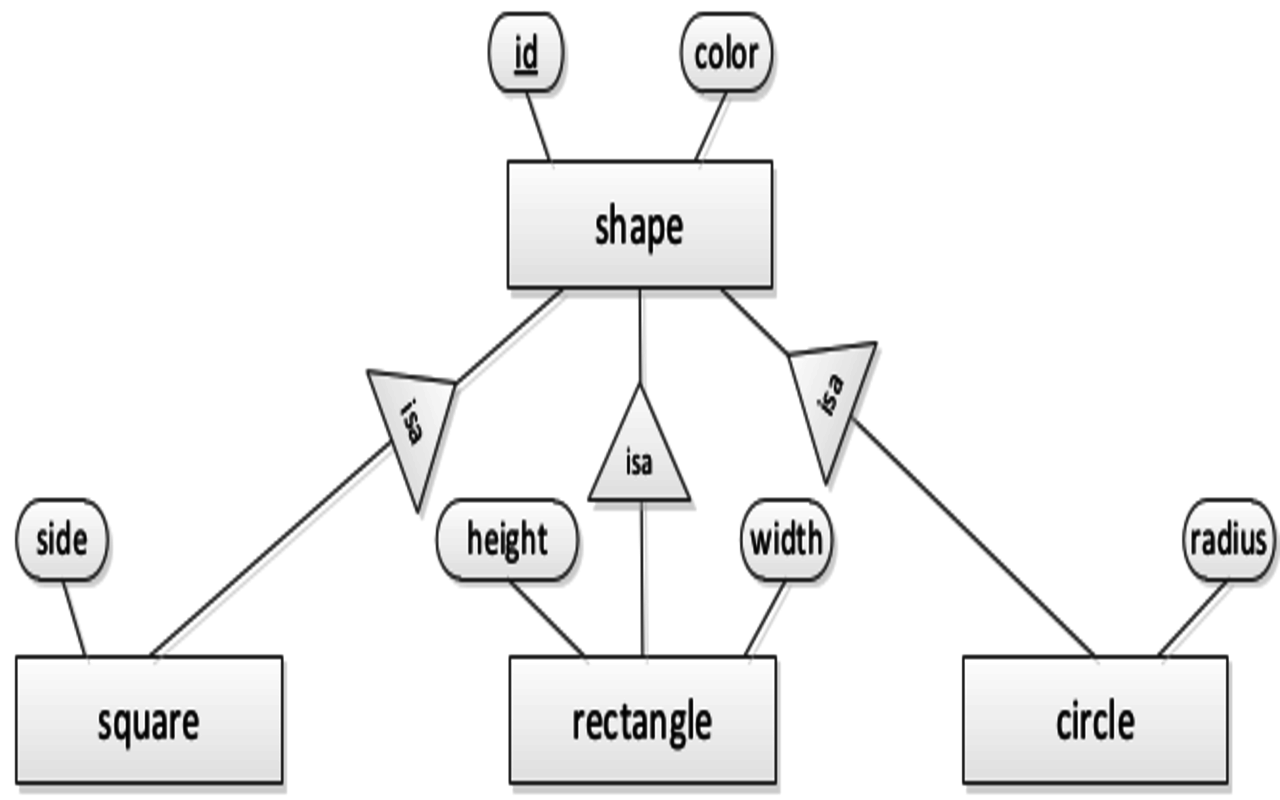
\includegraphics[scale=0.3]{11.PNG}
\subsection*{5.1}
From the above E/R diagram make relational schemas using each of the following approaches
$$a)\: The\:straight\:E/R\:method.$$
Shape(\underline{id}, color)\\
Square(\underline{id}, side)\\
Rectangle(\underline{id}, height, width)\\
Circle(\underline{id}, radius)

$$b)\: The\:object-oriented\:method.$$
Shape(\underline{id}, color)\\
ShapeS(\underline{id}, color, side)\\
ShapeR(\underline{id}, color, height, width)\\
ShapeC(\underline{id}, color, radius)\\
ShapeSR(\underline{id}, color, side, height, width)

$$c)\: The\:null\:method.$$
Shape(\underline{id}, color, side, height, width, radius)

\subsection*{5.2}
Write the SQL statements that will modify data stored in the schemas from 5.1.
$$a)\: Add\:a\:new\:red\:circle\:with\:radius\:34\:and\:id\:1234$$
With the E/R method schema:\\
\\
INSERT INTO 	Shape\\
VALUES (1234, RED);\\
INSERT INTO Circle\\
VALUES (1234, 34);\\
\\
With the object-oriented method schema:\\
\\
INSERT INTO ShapeC\\
VALUES (1234, RED, 34);\\
\\
With the null method schema:\\
\\
INSERT INTO Shape
VALUES(1234, RED, NULL, NULL, NULL, 34);\\

$$b)\: Change\:the\:color\:to\:blue\:for\:the\:shape\:identified\:by\:id\:4321$$
With the E/R method schema:\\
\\
UPDATE Shape\\
SET color = BLUE\\
WHERE id = 4321;\\
\\
With the object-oriented method schema:\\
\\
UPDATE Shape\\
SET color = BLUE\\
WHERE id = 4321;\\
\\
UPDATE ShapeS\\
SET color = BLUE\\
WHERE id = 4321;\\
\\
UPDATE ShapeR\\
SET color = BLUE\\
WHERE id = 4321;\\
\\
UPDATE ShapeC\\
SET color = BLUE\\
WHERE id = 4321;\\
\\
UPDATE ShapeSR\\
SET color = BLUE\\
WHERE id = 4321;\\
\\
With the null method schema:\\
\\
UPDATE Shape\\
SET color = BLUE\\
WHERE id = 4321;\\

$$c)\: Delete\:all\:rectangles\:with\:a\:height\:between\:30\:and\:40.$$
These will delete rectangles with a height 'between' 30 and 40 and not rectangles with a height of exactly 30 or 40.\\
\\
With the E/R method schema:\\
\\
DELETE FROM Rectangle\\
WHERE height $>$ 30 AND height $<$ 40;\\
\\
With the object-oriented method schema:\\
\\
DELETE FROM ShapeR\\
WHERE height $>$ 30 AND height $<$ 40;\\
\\
With the null method schema:\\
\\
DELETE FROM Shape\\
WHERE height $>$ 30 AND height $<$ 40;

\end{document}
